\documentclass[11pt,a4paper]{article}
% rozmery stranky
\usepackage[left=2cm,text={18cm, 25cm},top=3cm]{geometry}
% cestina a fonty
\usepackage[czech]{babel}
\usepackage[utf8]{inputenc}
\usepackage[T1]{fontenc}
\usepackage{times}
\usepackage{multirow}
% dalsi balicky
\usepackage{graphicx}
\usepackage{algorithm2e}
% TODO: projekt neni dokonceny
\begin{document}

  \begin{titlepage}
    \begin{center}
      \Huge\textsc{Vysoké učení technické v Brně} \\ 
      \huge\textsc{Fakulta informačních technologií} \\[84mm]
      \LARGE{Typografie a publikování \,--\, 3. projekt} \\
      \Huge{Tabulky a obrázky}
      \vfill
    \end{center}
    \Large{9. dubna 2014 \hfill Roman Blanco}
  \end{titlepage}
  \section{Úvodní strana}

    Název práce umístěte do zlatého řezu a nezapomeňte uvést dnešní datum a vaše jméno a příjmení.

  \section{Tabulky}

  Pro sázení tabulek můžeme použít buď prostředí \texttt{tabbing} nebo prostředí \texttt{tabular}.

    \subsection{Prostředí \texttt{tabbing}}

    Při použití \texttt{tabbing} vypadá tabulka následovně:

      \begin{tabbing}
        Vodní melouny ~~~~\= Cena ~~~~  \= 2,5 kg \kill
        \bfseries Ovoce \>
        \bfseries Cena \>
        \bfseries Množství \\
        Jablka \> 25,90 \> 3 kg \\
        Hrušky \> 27,40 \> 2,5 kg \\
        Vodní melouny \> 35,-- \> 1 kus
      \end{tabbing}


    Toto prostředí se dá také použít pro sázení algoritmů, ovšem vhodnější je použít prostředí \texttt{algorithm} nebo \texttt{algorithm2e} (viz sekce 3).
      % TODO sekce 3

    \subsection{Prostředí \texttt{tabular}}
    
      Další možností, jak vytvořit tabulku, je použít prostředí \texttt{tabular}. Tabulky pak budou vypadat takto\footnote{Kdyby byl problem s \texttt{cline}, zkuste se podívat třeba sem: : http://www.abclinuxu.cz/tex/poradna/show/325037.}:

   
        \begin{table}[h]
        \centering
        \catcode`\-=12
          \begin{tabular}{|l|c|c|}
            \hline
             & \multicolumn{2}{|c|}{Cena}  \\ 
            \cline{2-3}
            Měna & nákup & prodej \\
            \hline
            EUR & 27,34 & 27,42 \\
            GBP & 33,09 & 33,21 \\
            USD & 19,87 & 19,95 \\
            \hline

          \end{tabular}
          \caption{Tabulka kurzů k dnešnímu dni}

   % TODO tabulka 2

\end{table}
\pagebreak

  \section{Algoritmy}

  Pokud budeme chtít vysázet algoritmus, můžeme použít prostředí \texttt{algorithm}\footnote{Pro nápovědu, jak zacházet s prostředím \texttt{algorithm}, můžeme zkusit tuhle stránku: \\http://ftp.cstug.cz/pub/tex/CTAN/macros/latex/contrib/algorithms/algorithms.pdf.} nebo \texttt{algorithm2e}\footnote{Pro \texttt{algorithm2e} zase tuhle: http://ftp.cstug.cz/pub/tex/CTAN/macros/latex/contrib/algorithm2e/algorithm2e.pdf.}. Příklad použití prostředí \texttt{algorithm2e} viz Algoritmus 1.

   
    \vspace*{-0.15cm}
    \IncMargin{1.2em}
    \begin{algorithm}
      \SetAlgoNoLine
      \SetNlSkip{0em}
      \SetNlSty{normal}{}{:}
      \SetKwInput{Input}{Input}
      \SetKwInOut{Output}{Output}
      \SetKwFor{For}{for}{do}{end\,for}
    \Indm  
        \Input{$(X_{t-1},u_t,z_t)$}
        \Output{$X_t$} 
    \Indp
    \Indp
      \BlankLine
      $\overline{X_t} = X_t = 0$ \BlankLine   
      \For{$k = 1$ to $M$}{   
        $x_t^{[k]} = sample\_motion\_model(u_t, x_{t-1}^{[k]})$\\
        $\omega_t^{[k]} = measuremen\_model(z_t, x_{t}^{[k]}, m_{t-1})$\\
        $m_t^{[k]} = updated\_occupancy\_grid(z_t, x_{t}^{[k]}, m_{t-1}^{[k]})$\\
        $\overline{X_t} = \overline{X_t} + \langle x_x^{[m]},\omega_t^{[m]} \rangle $
      }
      
      \For{$k = 1$ to $M$}{   
        draw $i$ with probability $\approx \omega_t^{[i]}$\\
        add $\langle x_x^{[k]},m_t^{[k]} \rangle$ to $X_t$
      }
      \Return{$X_t$}
            
    \caption{\textsc{Fast}SLAM}
    \end{algorithm}
    \DecMargin{1.2em}

  \section{Obrázky}

      Do našich článků můžeme samozřejmě vkládat obrázky. Pokud je obrázkem fotografie, můžeme klidně použít bitmapový soubor. Pokud by to ale mělo být nějaké schéme nebo něco podobného, je dobrým zvykem takovýto obrázek vytvořit vektorově.
    \begin{figure}[ht]
  \begin{center}
    \scalebox{0.4}{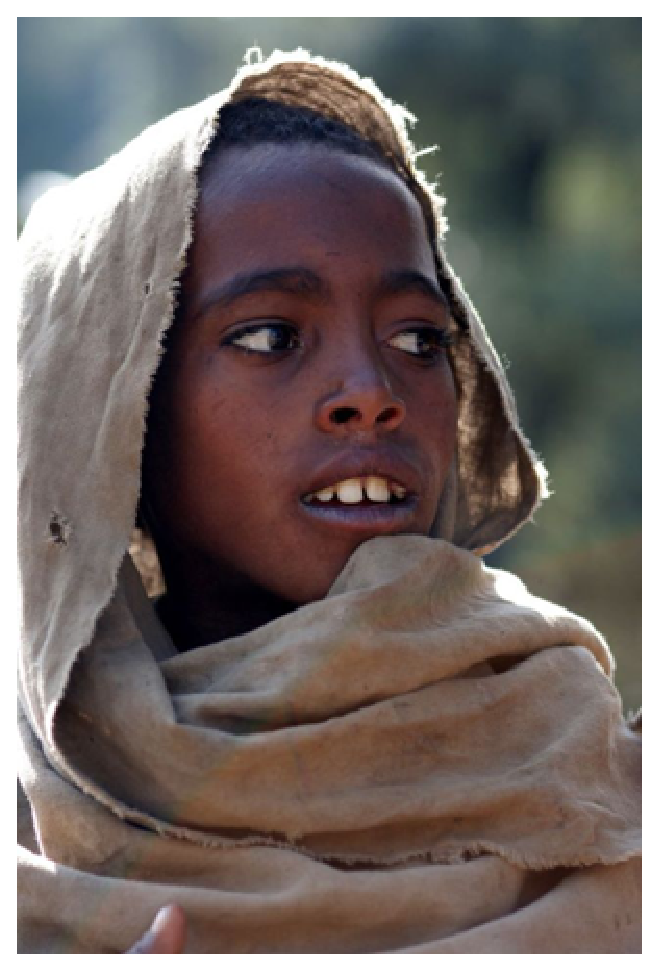
\includegraphics{etiopan.eps}
    \reflectbox{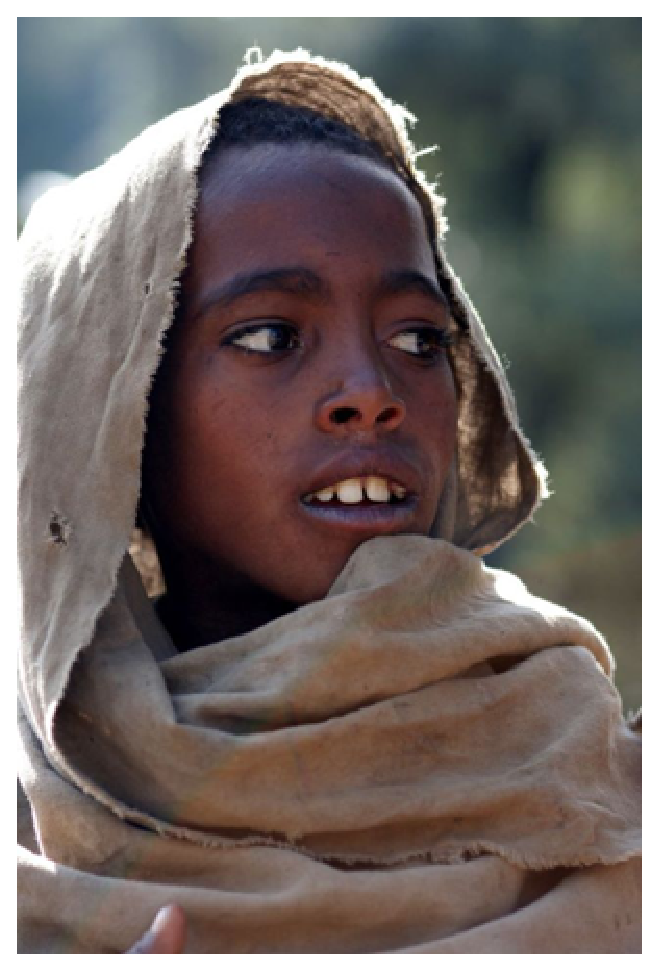
\includegraphics{etiopan.eps}} }
    \caption{Malý etiopánek a jeho bratříček}
  \end{center}
\end{figure}

 \newpage
Rozdíl mezi vektorovým...

\begin{figure}[ht]
  \begin{center}
    \scalebox{0.4}{
\includegraphics{oniisan.eps}}
    \caption{Vektorový obrázek}
  \end{center}
\end{figure}


... a bitmapovým obrázkem


\begin{figure}[ht]
  \begin{center}
    \scalebox{0.6}{
\includegraphics{oniisan2.eps}}
    \caption{Bitmapový obrázek}
  \end{center}
\end{figure}


se projeví například při zvětšení.

Odkazy (nejen ty) na obrázky 1, 2 a 3, na tabulky 1 a 2 a také na algoritmus 1 jsou udělány pomocí křížových odkazů. Pak je ovšem potřeba zdrojový soubor přeložit dvakrát.

Vektor obrázky lze vytvořit i přímo v \LaTeX u, například pomocí prostředí \texttt{picture}. Všechny rozměry jsou uváděny v mm.

\newpage

  \begin{figure}
    \begin{center}
    \setlength{\unitlength}{1.35mm}
    \begin{picture}(115,158.5)
    \put(0,0){\linethickness{1pt}\framebox(115,158.5){}}
      \put(91,145){\makebox(15,14.5){\shortstack{Výška \\ mezery\,=\,14,5}}}
      \put(88,151.25){\vector(0,1){7.25}}
      \put(88,151.25){\vector(0,-1){7.25}}
      \put(89,132){\makebox(15,14.5){\shortstack{Výška \\ mezery\,=\,10}}}
      \put(88,139){\vector(0,1){5}}
      \put(88,139){\vector(0,-1){5}}
      \put(90,122){\makebox(15,14.5){\shortstack{Výška \\ hlavičky\,=\,10}}}
      \put(88,129){\vector(0,1){5}}
      \put(88,129){\vector(0,-1){5}}
      \put(89,110){\makebox(15,14.5){\shortstack{Výška \\ mezery\,=\,14}}}
      \put(88,117){\vector(0,1){7}}
      \put(88,117){\vector(0,-1){7}}
      \put(94,77.5){\linethickness{1pt}\framebox(15,10){\textbf{\shortstack{Okrajová\\ poznámka}}}}
      \put(92,88){\makebox(20,14.5){\shortstack{Šířka\\ boxu\,=\,15}}}
      \put(102,91.5){\vector(-1,0){7.5}}
      \put(102,91.5){\vector(1,0){7.5}}
      \put(87.5,97.5){\makebox(20,14.5){\shortstack{Mezera\,=\,9}}}
      \put(94,103.5){\vector(-1,-3){4}}
      \put(90,91.5){\vector(-1,0){4.5}}
      \put(90,91.5){\vector(1,0){4.5}}
      \put(87.5,57){\makebox(15,14.5){\shortstack{Výška\\ těla\,=\,75}}}
      \put(88,72.5){\vector(0,1){37.5}}
      \put(88,72.5){\vector(0,-1){37.5}} 
      \put(89.5,19){\makebox(15,14.5){\shortstack{Výška\\ mezery\,=\,15}}}
      \put(88,27.5){\vector(0,1){7.5}}
      \put(88,27.5){\vector(0,-1){7.5}}  
      \put(88,6){\makebox(15,14.5){\shortstack{Výška\\ paty\,=\,10}}}
      \put(88,15){\vector(0,1){5}}
      \put(88,15){\vector(0,-1){5}}  
      \put(53,3){\makebox(10,5){\shortstack{Šířka stránky = 115}}}
      \put(57.5,3){\vector(1,0){57.5}}
      \put(57.5,3){\vector(-1,0){57.5}}
      \put(94,43){\makebox(15,14.5){\shortstack{Výška\\ stránky\,=\,158,5}}}
      \put(102,55){\vector(1,1){10}}
      \put(112,79.25){\vector(0,1){79.25}}
      \put(112,79.25){\vector(0,-1){79.25}}
      \multiput(15,151.5)(0,-10){16}{\line(0,1){7}}
      \multiput(0,144)(10,0){11}{\line(1,0){7}}   
      \put(2.5,91.5){\makebox(10,5){\shortstack{Mezera = 15}}}
      \put(7.5,91.5){\vector(1,0){7.5}}
      \put(7.5,91.5){\vector(-1,0){7.5}}
      \put(53,137){\makebox(10,5){\shortstack{Šířka boxu = 55}}}
      \put(57.5,137){\vector(1,0){27.5}}
      \put(57.5,137){\vector(-1,0){27.5}}
      \put(30,124){\linethickness{1pt}\framebox(55,10){\textbf{Hlavička}}}
      \put(30,35){\linethickness{1pt}\framebox(55,75){\textbf{Textové tělo}}}
      \put(30.5,10){\linethickness{1pt}\framebox(55,10){\textbf{Pata}}}
      \end{picture}
    \caption{Vektorový obrázek v~prostředí \texttt{picture}}
    \end{center}
  \end{figure}
\end{document}